\begin{ZhChapter}

\chapter{緒論}

\section{研究背景}

科技的快速進步,讓人們的生活更加便利,物聯網(IoT)的應用已經與日常生活密不可分,包含了醫療及工業的應用,無所不在,\cite{mordor2024iot}根據日商環球訊息有限公司(GII)調查,物聯網(IoT)市場規模預計從2024年到2029年,將從1.17兆美元增加至2.37兆美元,年均複合成長率(CAGR)為15.12\%,如圖\ref{fig: IoT市場規模評估}所示。

\begin{figure}[H]
    \centering
    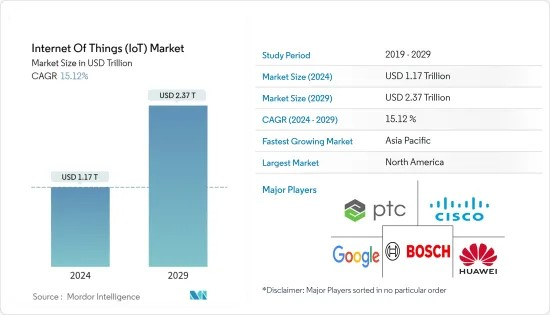
\includegraphics[width = 1\textwidth]{image/market_research.jpg}
    \caption{IoT市場規模評估\cite{mordor2024iot}}
    \label{fig: IoT市場規模評估}
\end{figure}

2010年6月藍牙技術聯盟(Bluetooth Special Interest Group)提出了低功耗藍牙(Bluetooth Low Energy, BLE),BLE省電及低成本的特性,使得藍牙技術在物聯網(IoT)的應用種佔據了不可或缺的角色,例如:目前市面上的無線設備包括藍牙耳機、藍牙鍵盤及藍牙滑鼠。
物聯網(IoT)的應用中,大量使用無線感測網路(Wireless Sensor Networks, WSN),會在環境之中分布許多的節點,而節點不只有當作感知器測量環境的數據,常常還要當作中繼節點,轉傳發送端與目的端的封包,最終將所有量測的數據匯集到終端節點,以監控所有的節點數據,將數據儲存後,進行分析後並做出適當的處理,也可以透過分析數據預測環境的變化,並提前做出適當的處理。

藍牙網狀網路(Bluetooth Mesh)架構的實現,讓BLE更具有可靠性(Reliability)及擴展性(Scalability),可以允許多個BLE裝置相互連接並形成網狀結構,讓封包可以在多個裝置之間進行傳輸,讓傳輸距離不會受到單一裝置的傳輸範圍限制,解決了節點之間裝置連接數量的限制以及傳輸距離不足的問題,在物聯網(IoT)的應用,例如:智慧建築、智慧工業、智慧城市、智慧家庭..等等,BLE都已經扮演重要也不可或缺的角色。
	
%在物聯網(IoT)與藍牙網狀網路(Bluetooth Mesh)中,對整個系統架構做出適當的評估,在不影響裝置效能的情況下,設計多個藍牙裝置之間的分流機制,因為在整個系統中,流量可能會有所起伏,為了讓每個裝置可以有一樣的傳輸品質,且系統可以發揮最好的吞吐量。
	

\section{研究動機與目的}

FruityMesh是一個專門為BLE Mesh Network所開發的開源網路協定框架。在文獻\cite{112TIT00392032}中的研究,發現在原生FruityMesh上封包傳輸是採用廣播的方式,向相鄰的所有節點發送封包,這種設計雖然簡單,卻容易導致大量冗餘封包的產生,這會導致節點之間傳輸不必要的封包,最終導致整個BLE Mesh出現廣播風暴。因此\cite{112TIT00392032}作者針對FruityMesh傳輸時產生的廣播風暴,提出了DOT(Destination Oriented Transmission)排程的機制,將BLE Mesh導入樹狀結構,對整個系統進行分層管理,讓封包傳輸只會向目的端正確的路徑上傳輸,避免了廣播風暴的產生。作者在研究過程中,也發現BLE Multi-Hop網狀網路節點會擁有Master以及Slave兩種角色,而在同一個時間下,節點同時會是Master和Slave的狀態,而這種狀態上的衝突會導致的封包傳輸產生遺失現象。

\cite{112TIT00392032}作者為了解決角色衝突的問題,在DOT的架構下增加啟用以及禁用的機制,提出DOST(Destination Oriented Switch Transmission)的排程設計,利用時間交錯方式讓裝置在同一個時間只會扮演Master或Slave,解決在同一個時間點節點可能會因為扮演Master及Slave角色衝突而導致的封包傳輸遺失的問題;因此,在FruityMesh中導入DOST設計後已經改善了大部分的封包傳輸延遲以及封包重傳率,但仍存在些許效能瓶頸,因為在無線網路中,所有節點的封包傳輸都是透過無線電波,以廣播的方式傳輸,這會導致在多個節點同時傳輸封包時,可能會產生封包碰撞的問題,導致封包傳輸延遲增加。


此外,\cite{112TIT00392032}文獻指出,若要在 DOST 架構下進一步提升效能,需確保拓樸建立時,Sink 節點為整體網路的根節點。然而原研究並未針對拓樸控制機制提出具體解法。若未能確保 Sink 位於樹根,當其斷線並重新加入網路時,可能無法恢復為原先的根節點角色,進而影響整體傳輸路徑的穩定性與效能。

在\cite{112TIT00392032}\cite{110TIT00392037}中,針對了single hop mesh 及 multi hop mesh的網路拓樸進行探討,當使用合適的封包連接參數可以有效降低封包傳輸延遲及重傳率;\cite{109TIT00392031}中,探討了在不同封包大小的情形下,計算出最適合的連接參數,在傳輸過程動態調整連接的CE(Connection Event)及CI(Connection Interval),達到更好的吞吐量。

本計畫將研究中在DOT的排程設計下,仍然會有些許因為封包遺失,而產生的封包重傳的問題,以及在藍牙網狀網路(Bluetooth Mesh)架構,執行TDMA的排程機制,結合調整連線參數,確保傳輸品質,並修改FruityMesh拓樸方法,讓BLE Mesh建立的過程確保Sink點在整個樹狀結構的根節點,也確保Sink點如果斷線後重新連線後依然是整個BLE Mesh樹狀結構的根節點。

\section{論文架構}
本論文共分為五章,第一章說明本研究的背景與動機,並闡述本論文所要解決的問題與研究目的。

第二章整理並探討本研究所依據的基礎知識與技術背景,包括藍牙低功耗(BLE)通訊技術、藍牙網狀網路(BLE Mesh)架構、BLE 中的排程與連線機制(如 CI、CE)、以及目的地傾向傳輸策略。此外,也介紹本研究所採用的開發平台,包含 Nordic Semiconductor 所推出的 nRF52840 晶片與 SoftDevice 堆疊,以及基於該硬體的 FruityMesh 開源框架,並進一步說明 FruityMesh 的 Cluster 與 Self-Healing 機制。

第三章分析現有 FruityMesh 在拓樸建立與封包傳輸上可能出現的問題。接著提出改良的拓樸建立演算法與設計,包括以 Master 或 Slave 身分進行最佳連線選擇,以及改善自我修復(Self-Healing)行為的拓樸重建機制。此外,本章亦設計改善封包傳輸效能的對應策略,以確保在多節點環境下依然能維持高效通訊。

第四章說明本研究之實驗設計與評估方式,分別建置實體測試平台與模擬平台(CheerySim)以模擬不同節點規模下的網路拓樸生成與封包傳輸行為。實驗部分以多組節點數模擬進行測試,並設計多項效能評估指標,包括拓樸建立時間、自我修復時間、平均 HopsToSink 數值、封包傳輸延遲、封包抵達率與封包重傳率,藉此全面評估所提出機制的實際效能表現。

第五章總結本研究的成果與貢獻,並探討未來在 BLE Mesh 網路設計中可延伸的研究方向與改進空間,期望能為低功耗網狀通訊領域提供可參考之實作架構與演算法設計依據。


\end{ZhChapter}